% Author: Izaak Neutelings (August, 2017)

\documentclass[border=3pt,tikz]{standalone} %[dvipsnames]

\usepackage{amsmath} % for \dfrac
\usepackage{tikz}
\tikzset{>=latex} % for LaTeX arrow head
\usepackage{pgfplots} % for the axis environment
\usepackage{xcolor}
\usepackage[outline]{contour} % halo around text
\contourlength{1.2pt}
\usetikzlibrary{positioning,calc}
\usetikzlibrary{backgrounds}% required for 'inner frame sep'
%\usepackage{adjustbox} % add whitespace (trim)

% define gaussian pdf and cdf
\pgfmathdeclarefunction{gauss}{3}{%
  \pgfmathparse{1/(#3*sqrt(2*pi))*exp(-((#1-#2)^2)/(2*#3^2))}%
}
\pgfmathdeclarefunction{cdf}{3}{%
  \pgfmathparse{1/(1+exp(-0.07056*((#1-#2)/#3)^3 - 1.5976*(#1-#2)/#3))}%
}
\pgfmathdeclarefunction{fq}{3}{%
  \pgfmathparse{1/(sqrt(2*pi*#1))*exp(-(sqrt(#1)-#2/#3)^2/2)}%
}
\pgfmathdeclarefunction{fq0}{1}{%
  \pgfmathparse{1/(sqrt(2*pi*#1))*exp(-#1/2))}%
}

\colorlet{mydarkblue}{blue!30!black}

% to fill an area under function
\usepgfplotslibrary{fillbetween}
\usetikzlibrary{patterns}
\pgfplotsset{compat=1.12} % TikZ coordinates <-> axes coordinates
% https://tex.stackexchange.com/questions/240642/add-vertical-line-of-equation-x-2-and-shade-a-region-in-graph-by-pgfplots

% plot aspect ratio
%\def\axisdefaultwidth{8cm}
%\def\axisdefaultheight{6cm}

% number of sample points
\def\N{50}
\begin{document}






% GAUSSIANs: basic properties
\begin{tikzpicture}
  
  \def\B{11};
  \def\Bs{3.0};
  \def\xmax{\B+3.2*\Bs};
  \def\ymin{{-0.1*gauss(\B,\B,\Bs)}};
  \def\h{0.07*gauss(\B,\B,\Bs)};
  \def\a{\B-0.8*\Bs};
  
  \begin{axis}[every axis plot post/.append style={
               mark=none,domain={-0.05*(\xmax)}:{1.08*\xmax},samples=\N,smooth},
               xmin={-0.1*(\xmax)}, xmax=\xmax,
               ymin=\ymin, ymax={1.1*gauss(\B,\B,\Bs)},
               axis lines=middle,
               axis line style=thick,
               enlargelimits=upper, % extend the axes a bit to the right and top
               ticks=none,
               xlabel=$x$,
               every axis x label/.style={at={(current axis.right of origin)},anchor=north},
               width=0.7*\textwidth, height=0.55*\textwidth,
               y=700pt,
               clip=false
              ]
    
    % PLOTS
    \addplot[blue,thick,name path=B] {gauss(x,\B,\Bs)};
    
    % FILL
    \path[name path=xaxis]
      (0,0) -- (\pgfkeysvalueof{/pgfplots/xmax},0);
    \addplot[blue!25] fill between[of=xaxis and B, soft clip={domain=-1:{\a}}];
    
    % LINES
    \addplot[mydarkblue,dashed,thick]
      coordinates {({\a},{1.2*gauss(\a,\B,\Bs)}) ({\a},{-\h})}
      node[mydarkblue,below=-2pt] {$a$};
    \node[mydarkblue,above right] at ({\B+\Bs},{1.2*gauss(\B+\Bs,\B,\Bs)}) {$f(x)$};
    \node[blue!60!black,above left] at ({0.85*(\a)},{1.0*gauss(0.85*(\a),\B,\Bs)}) {$P(X\leq a)$};
    
  \end{axis}
\end{tikzpicture}



% GAUSSIANs: basic properties
\begin{tikzpicture}
  
  \def\B{11};
  \def\Bs{3.0};
  \def\xmax{\B+3.2*\Bs};
  \def\ymin{{-0.1*gauss(\B,\B,\Bs)}};
  \def\h{0.1*gauss(\B,\B,\Bs)};
  
  \begin{axis}[every axis plot post/.append style={
               mark=none,domain={-0.05*(\xmax)}:{1.08*\xmax},samples=\N,smooth},
               xmin={-0.1*(\xmax)}, xmax=\xmax,
               ymin=\ymin, ymax={1.1*gauss(\B,\B,\Bs)},
               axis lines=middle,
               axis line style=thick,
               enlargelimits=upper, % extend the axes a bit to the right and top
               ticks=none,
               xlabel=$x$,
               every axis x label/.style={at={(current axis.right of origin)},anchor=north},
               width=0.85*\textwidth, height=0.55*\textwidth,
               y=700pt,
               clip=false
              ]
    
    % PLOTS
    \addplot[blue,thick,name path=B] {gauss(x,\B,\Bs)};
    
    % FILL
    \path[name path=xaxis]
      (0,0) -- (\pgfkeysvalueof{/pgfplots/xmax},0); %\pgfkeysvalueof{/pgfplots/xmin}
    \addplot[blue!50] fill between[of=xaxis and B, soft clip={domain={\B-3*\Bs}:{\B+3*\Bs}}];
    \addplot[blue!25] fill between[of=xaxis and B, soft clip={domain={\B-2*\Bs}:{\B+2*\Bs}}];
    \addplot[blue!10] fill between[of=xaxis and B, soft clip={domain={\B-1*\Bs}:{\B+1*\Bs}}];
    
    % LINES
    \addplot[black,dashed,thick]
      coordinates {({\B-3*\Bs},{18*gauss(\B-3*\Bs,\B,\Bs)}) ({\B-3*\Bs},{-\h})};
    \addplot[black,dashed,thick]
      coordinates {({\B-2*\Bs},{3*gauss(\B-2*\Bs,\B,\Bs)}) ({\B-2*\Bs},{-\h})};
    \addplot[black,dashed,thick]
      coordinates {({\B-1*\Bs},{1.2*gauss(\B-\Bs,\B,\Bs)}) ({\B-1*\Bs},{-\h})};
    \addplot[black,dashed,line width=0.7pt]
      coordinates {(\B,{1.05*gauss(\B,\B,\Bs)}) (\B,{-\h})};
    \addplot[black,dashed,thick]
      coordinates {({\B+1*\Bs},{1.2*gauss(\B+\Bs,\B,\Bs)}) ({\B+1*\Bs},{-\h})};
    \addplot[black,dashed,thick]
      coordinates {({\B+2*\Bs},{3*gauss(\B+2*\Bs,\B,\Bs)}) ({\B+2*\Bs},{-\h})};
    \addplot[black,dashed,thick]
      coordinates {({\B+3*\Bs},{18*gauss(\B+3*\Bs,\B,\Bs)}) ({\B+3*\Bs},{-\h})};
    
    % LABELS
    \node[below=-2pt,scale=0.8] at ({\B-3*\Bs},{-\h}) {\strut$\mu-3\sigma$};
    \node[below=-2pt,scale=0.8] at ({\B-2*\Bs},{-\h}) {\strut$\mu-2\sigma$};
    \node[below=-2pt,scale=0.8] at ({\B-\Bs},{-\h}) {\strut$\mu-\sigma$};
    \node[below=-2pt,scale=0.8] at (\B,{-\h}) {\strut$\mu$};
    \node[below=-2pt,scale=0.8] at ({\B+\Bs},{-\h}) {\strut$\mu+\sigma$};
    \node[below=-2pt,scale=0.8] at ({\B+2*\Bs},{-\h}) {\strut$\mu+2\sigma$};
    \node[below=-2pt,scale=0.8] at ({\B+3*\Bs},{-\h}) {\strut$\mu+3\sigma$};
    
    % AREAS
    \addplot[<->,mydarkblue,thick]
      coordinates {({\B-\Bs},{.55*gauss(\B,\B,\Bs)}) ({\B+\Bs},{.55*gauss(\B,\B,\Bs)})};
    \addplot[<->,mydarkblue,thick]
      coordinates {({\B-2*\Bs},{.35*gauss(\B,\B,\Bs)}) ({\B+2*\Bs},{.35*gauss(\B,\B,\Bs)})};
    \addplot[<->,mydarkblue,thick]
      coordinates {({\B-3*\Bs},{.15*gauss(\B,\B,\Bs)}) ({\B+3*\Bs},{.15*gauss(\B,\B,\Bs)})};
    \node[mydarkblue,fill=blue!10,inner xsep=3,inner ysep=1,scale=1]
      at (\B,{.55*gauss(\B,\B,\Bs)}) {68.3\%};
    \node[mydarkblue,fill=blue!10,inner xsep=3,inner ysep=2,scale=1]
      at (\B,{.35*gauss(\B,\B,\Bs)}) {95.5\%};
    \node[mydarkblue,fill=blue!10,inner xsep=3,inner ysep=2,scale=1]
      at (\B,{.15*gauss(\B,\B,\Bs)}) {99.7\%};
    
  \end{axis}
\end{tikzpicture}



% GAUSSIANs: error bands
\begin{tikzpicture}
  
  \def\B{10};
  \def\Bs{3.0};
  \def\xmax{\B+3.2*\Bs};
  \def\ymin{{-0.15*gauss(\B,\B,\Bs)}};
  
  \begin{axis}[every axis plot post/.append style={
               mark=none,domain={-0.05*(\xmax)}:{1.08*\xmax},samples=\N,smooth},
               xmin={-0.1*(\xmax)}, xmax=\xmax,
               ymin=\ymin, ymax={1.1*gauss(\B,\B,\Bs)},
               axis lines=middle,
               axis line style=thick,
               enlargelimits=upper, % extend the axes a bit to the right and top
               ticks=none,
               xlabel=$-2\ln Q$, %q
               every axis x label/.style={at={(current axis.right of origin)},anchor=north},
               width=0.7*\textwidth, height=0.5*\textwidth,
               y=700pt
              ]
    
    % PLOTS
    \addplot[blue, name path=B,thick] {gauss(x,\B,\Bs)};
    \addplot[black,dashed,thick]
      coordinates {({\B-2*\Bs}, {0.60*gauss(\B,\B,\Bs)}) ({\B-2*\Bs}, \ymin)};
    \addplot[black,dashed,thick]
      coordinates {({\B-1*\Bs}, {0.90*gauss(\B,\B,\Bs)}) ({\B-1*\Bs}, \ymin)};
    \addplot[black,dashed,line width=0.7pt]
      coordinates {(\B, {1.10*gauss(\B,\B,\Bs)}) (\B,\ymin)};
    \addplot[black,dashed,thick]
      coordinates {({\B+1*\Bs}, {0.90*gauss(\B,\B,\Bs)}) ({\B+1*\Bs}, \ymin)};
    \addplot[black,dashed,thick]
      coordinates {({\B+2*\Bs}, {0.60*gauss(\B,\B,\Bs)}) ({\B+2*\Bs}, \ymin)};
    
    \node[above=-2pt] at ({\B-1.5*\Bs},\ymin) {\small$-2\sigma$};
    \node[above=-2pt] at ({\B-0.5*\Bs},\ymin) {\small$-1\sigma$};
    \node[above=-2pt] at ({\B+0.5*\Bs},\ymin) {\small$+1\sigma$};
    \node[above=-2pt] at ({\B+1.5*\Bs},\ymin) {\small$+2\sigma$};
    
    % FILL
    \path[name path=xaxis]
      (0,0) -- (\pgfkeysvalueof{/pgfplots/xmax},0); %\pgfkeysvalueof{/pgfplots/xmin}
    \addplot[black!0!yellow] fill between[of=xaxis and B, soft clip={domain={\B-2*\Bs}:{\B+2*\Bs}}];
    \addplot[black!10!green] fill between[of=xaxis and B, soft clip={domain={\B-1*\Bs}:{\B+1*\Bs}}];
    
    % LABELS
    %\node[above=0pt, black!20!blue] at (\B,{1.05*gauss(\B,\B,\Bs)}) {$f(x|\text{b})$};
    %\node[] at ($(\ymin,0)!0.5!(\ymin,0)$) {$+2\sigma$};
    
  \end{axis}
\end{tikzpicture}



% GAUSSIANs: confidence level
\begin{tikzpicture}
  
  \def\q{5};
  \def\B{3};
  \def\S{8};
  \def\Bs{1.0};
  \def\Ss{1.5};
  \def\xmax{\S+3.2*\Ss};
  \def\ymin{{-0.15*gauss(\B,\B,\Bs)}};
  
  \begin{axis}[every axis plot post/.append style={
               mark=none,domain={-0.05*(\xmax)}:{1.08*\xmax},samples=\N,smooth},
               xmin={-0.1*(\xmax)}, xmax=\xmax,
               ymin=\ymin, ymax={1.1*gauss(\B,\B,\Bs)},
               axis lines=middle,
               axis line style=thick,
               enlargelimits=upper, % extend the axes a bit to the right and top
               ticks=none,
               xlabel=$t$,
               every axis x label/.style={at={(current axis.right of origin)},anchor=north west},
               y=250pt
              ]
    
    % PLOTS
    \addplot[name path=B,thick,black!10!blue] {gauss(x,\B,\Bs)};
    \addplot[name path=S,thick,black!10!red ] {gauss(x,\S,\Ss)};
    \addplot[black,dashed,thick]
      coordinates {(\q, {0.95*gauss(\B,\B,\Bs)}) (\q, \ymin)}
      node[below=2pt,anchor=south west] {$t_\text{cut}$};
    \draw[->,thick]
      (\q,{0.90*gauss(\B,\B,\Bs)}) -- ({\q+1.6*\Ss},{0.90*gauss(\B,\B,\Bs)})
      node[above=4pt] {\footnotesize\qquad\qquad\qquad CRITICAL REGION};
    
    % FILL
    \path[name path=xaxis]
      (0,0) -- (\xmax,0);
    \addplot[white!50!blue] fill between[of=xaxis and B, soft clip={domain=\q:\xmax}];
    \addplot[white!50!red]  fill between[of=xaxis and S, soft clip={domain=0:\q}];
    
    % LABELS
    \node[above=2pt,  black!20!blue] at (       \B,      {gauss(\B,\B,\Bs)})     {$f(t|H_0)$};
    \node[above right,black!20!red ] at ({1.05*(\S+\Ss)},{gauss(\S+\Ss,\S,\Ss)}) {$f(t|H_1)$};
    \node[left, black!20!red, scale=1.3] at ({0.88*\q},{gauss(1.0*\q,\B,\Bs)}) {\strut$\beta$};
    \node[right,black!20!blue,scale=1.3] at ({1.12*\q},{gauss(1.0*\q,\B,\Bs)}) {\strut$\alpha$};
    \node[below=2pt] at ($(0,0)!0.4!(\q,0)$)     {ACCEPT};
    \node[below=2pt] at ($(\q,0)!0.6!(\xmax,0)$) {REJECT};
    
  \end{axis}
\end{tikzpicture}



% GAUSSIANs: p-value
\begin{tikzpicture}[inner frame sep=0]
  
  \def\q{5};
  \def\B{3};
  \def\S{8};
  \def\Bs{1.0};
  \def\Ss{1.5};
  \def\xmax{\B+3.2*\Bs};
  \def\ymin{{-0.15*gauss(\B,\B,\Bs)}};
  
  \begin{axis}[every axis plot post/.append style={
               mark=none,domain={-0.05*(\xmax)}:{1.08*\xmax},samples=\N,smooth},
               xmin={-0.1*(\xmax)}, xmax=\xmax,
               ymin=\ymin, ymax={1.1*gauss(\B,\B,\Bs)},
               axis lines=middle,
               axis line style=thick,
               enlargelimits=upper, % extend the axes a bit to the right and top
               ticks=none,
               xlabel=$t$,
               every axis x label/.style={at={(current axis.right of origin)},anchor=north west},
               y=250pt
              ]
    
    % PLOTS
    \addplot[name path=B,thick,black!10!blue] {gauss(x,\B,\Bs)};
    %\addplot[name path=S,thick,black!10!red ] {gauss(x,\S,\Ss)};
    \addplot[black,dashed,thick]
      coordinates {(\q,{-0.03*gauss(\B,\B,\Bs)}) (\q, {4.0*gauss(\q,\B,\Bs)})}
      node[below=-2pt,pos=0] {$t_\text{obs}$};
    
    % FILL
    \path[name path=xaxis]
      (0,0) -- (\xmax,0);
    \addplot[white!50!blue] fill between[of=xaxis and B, soft clip={domain=\q:\xmax}];
    
    % LABELS
    \node[above=2pt,  black!20!blue] at (       \B,      {gauss(\B,\B,\Bs)})     {$f(t|H_0)$};
    %\node[above right,black!20!red ] at ({1.05*(\S+\Ss)},{gauss(\S+\Ss,\S,\Ss)}) {$f(t|H_1)$};
    \node[left,black!20!blue,scale=1.3] at ({0.98*\q},{0.5*gauss(\q,\B,\Bs)}) {$p$};
    
  \end{axis}
\end{tikzpicture}



% GAUSSIANs: p-value, PLR
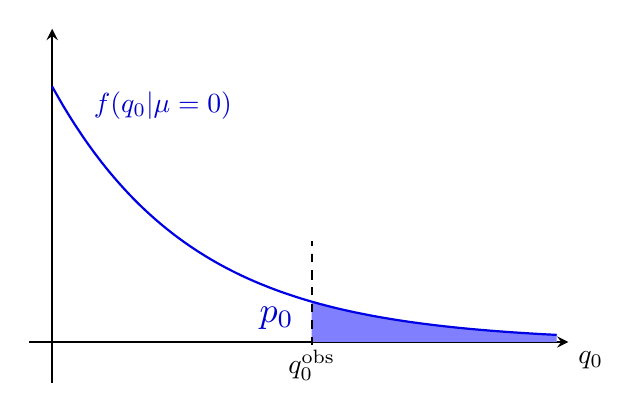
\begin{tikzpicture}
  
  \def\q{4.8}
  \def\Bs{2.6}
  \def\xmax{1.8*\q}
  \def\ymin{{-0.16/\Bs}}
  \def\ymax{{1.1/\Bs}}
  
  \begin{axis}[every axis plot post/.append style={
               mark=none,domain=0:{1.08*\xmax},samples=\N,smooth},
               xmin={-0.05*(\xmax)}, xmax=\xmax,
               ymin=\ymin, ymax=\ymax,
               axis lines=middle,
               axis line style=thick,
               enlargelimits=upper, % extend the axes a bit to the right and top
               ticks=none,
               xlabel=$q_0$,
               every axis x label/.style={at={(current axis.right of origin)},anchor=north west},
               y=240pt,
               domain=0:(\xmax)
              ]
    
    % PLOTS
    \addplot[name path=B,thick,black!10!blue] {exp(-x/\Bs)/\Bs};
    \addplot[black,dashed,thick]
      coordinates {(\q,{-0.08*exp(-\q/\Bs)/\Bs}) (\q, {2.5*exp(-\q/\Bs)/\Bs})}
      node[below=-2pt,pos=0] {$q_0^\text{obs}$};
    
    % FILL
    \path[name path=xaxis]
      (0,0) -- (1.08*\xmax,0);
    \addplot[white!50!blue] fill between[of=xaxis and B, soft clip={domain=\q:1.08*\xmax}];
    
    % LABELS
    \node[above right=2pt,black!20!blue] at ( 0.2*\Bs,{exp(-0.2)/\Bs}) {$f(q_0|\mu=0)$};
    \node[left,black!20!blue,scale=1.3] at ({0.98*\q},{0.6*exp(-\q/\Bs)/\Bs}) {$p_0$};
    
  \end{axis}
\end{tikzpicture}



% GAUSSIANs: p-value, PLR f(q|mu)
\begin{tikzpicture}
  
  \def\q{4.8}
  \def\S{1}
  \def\Ss{\S*0.35}
  \def\xmax{20}
  \def\ymin{-0.05}
  \def\ymax{0.5}
  
  \begin{axis}[every axis plot post/.append style={
               mark=none,domain=0:{1.08*\xmax},samples=\N,smooth},
               xmin={-0.05*\xmax}, xmax=\xmax,
               ymin=\ymin, ymax=\ymax,
               axis lines=middle,
               axis line style=thick,
               enlargelimits=upper, % extend the axes a bit to the right and top
               ticks=none,
               xlabel=$q_0$,
               every axis x label/.style={at={(current axis.right of origin)},anchor=north west},
               y=240pt,
               domain=0:(\xmax)
              ]
    
    % PLOTS
    \addplot[name path=B,thick,black!10!blue] {fq0(x)};
    \addplot[name path=B,thick,black!10!red] {fq(x,\S,\Ss)};
    
  \end{axis}
\end{tikzpicture}



% GAUSSIANs: expected sensitivity / p-value
\begin{tikzpicture}
  
  \def\q{4.8}
  \def\Bs{2.6}
  \def\S{\q}
  \def\Ss{1.4}
  \def\xmax{1.8*\q}
  \def\ymin{{-0.16/\Bs}}
  \def\ymax{{1.1/\Bs}}
  
  \begin{axis}[every axis plot post/.append style={
               mark=none,domain=0:{1.08*\xmax},samples=\N,smooth},
               xmin={-0.05*(\xmax)}, xmax=\xmax,
               ymin=\ymin, ymax=\ymax,
               axis lines=middle,
               axis line style=thick,
               enlargelimits=upper, % extend the axes a bit to the right and top
               ticks=none,
               xlabel=$q$,
               every axis x label/.style={at={(current axis.right of origin)},anchor=north west},
               y=240pt,
               domain=0:(\xmax)
              ]
    
    % PLOTS
    \addplot[name path=B,thick,black!10!blue] {exp(-x/\Bs)/\Bs};
    \addplot[name path=S,thick,black!10!red ] {gauss(x,\S,\Ss)};
    \addplot[black,dashed,thick]
      coordinates {(\q,{-0.08*exp(-\q/\Bs)/\Bs}) (\q, {1.08*gauss(\q,\S,\Ss)})}
      node[above right=-2pt] {$\text{Med}[q_0|\mu]$}
      node[below=-2pt,pos=0] {$q_0^\text{obs}$};
    
    % FILL
    \path[name path=xaxis]
      (0,0) -- (1.08*\xmax,0);
    \addplot[white!50!blue] fill between[of=xaxis and B, soft clip={domain=\q:1.08*\xmax}];
    
    % LABELS
    \node[above right=2pt,black!20!blue] at ( 0.2*\Bs,{exp(-0.2)/\Bs}) {$f(q_0|\mu=0)$};
    \node[above right=2pt,black!20!red] at ({1.3*\q},{gauss(1.3*\q,\S,\Ss)}) {$f(q_0|\mu)$};
    \node[left,black!20!blue,scale=1.3] at ({0.98*\q},{0.6*exp(-\q/\Bs)/\Bs}) {$p_0$};
    
  \end{axis}
\end{tikzpicture}



% GAUSSIANs: bias, variance
\begin{tikzpicture}[inner frame sep=0]
  
  \def\B{8};
  \def\T{4};
  \def\V{4};
  \def\Bs{1.0};
  \def\Ts{1.0};
  \def\Vs{2.0};
  \def\xmax{\B+3.2*\Bs};
  \def\ymin{{-0.15*gauss(\B,\B,\Bs)}};
  \def\ymax{{1.1*gauss(\B,\B,\Bs)}};
  
  \begin{axis}[every axis plot post/.append style={
               mark=none,domain={-0.05*(\xmax)}:{1.08*\xmax},samples=\N,smooth},
               xmin={-0.1*(\xmax)}, xmax=\xmax,
               ymin=\ymin, ymax=\ymax,
               axis lines=middle,
               axis line style=thick,
               enlargelimits=upper, % extend the axes a bit to the right and top
               ticks=none,
               xlabel=$\hat{\theta}$,
               ylabel={$f(\hat{\theta}|\theta)$},
               every axis x label/.style={at={(current axis.right of origin)},anchor=north west},
               every axis y label/.style={at={(current axis.above origin)},anchor=north east,align=center},
               y=200pt
              ]
    
    % PLOTS
    \addplot[name path=B,thick,black!10!blue ] {gauss(x,\B,\Bs)};
    \addplot[name path=S,thick,black!10!green] {gauss(x,\T,\Ts)};
    \addplot[name path=S,thick,black!10!red  ] {gauss(x,\V,\Vs)};
    \addplot[black,dashed,thick]
      coordinates {(\T,{-0.03*gauss(\T,\T,\Ts)}) (\T, {1.1*gauss(\T,\T,\Ts)})}
      node[below=-2pt,pos=0] {$\theta$};
    
%    % FILL
%    \path[name path=xaxis]
%      (0,0) -- (\xmax,0);
%    \addplot[white!50!blue] fill between[of=xaxis and B, soft clip={domain=\q:\xmax}];
%    
%    % LABELS
%    \node[above=2pt,  black!20!blue] at (       \B,      {gauss(\B,\B,\Bs)})     {$f(t|H_0)$};
%    %\node[above right,black!20!red ] at ({1.05*(\S+\Ss)},{gauss(\S+\Ss,\S,\Ss)}) {$f(t|H_1)$};
%    \node[left,black!20!blue,scale=1.3] at ({0.98*\q},{0.5*gauss(\q,\B,\Bs)}) {$p$};
    
  \end{axis}
\end{tikzpicture}



% GAUSSIANs: broading from nuisance parameter
\begin{tikzpicture}
  
  \def\B{3};
  \def\S{8};
  \def\Bs{1.0};
  \def\Bbs{1.2};
  \def\Ss{1.3};
  \def\Sbs{1.5};
  \def\xmax{\S+3.2*\Ss};
  \def\ymin{{-0.15*gauss(\B,\B,\Bbs)}};
  
  \begin{axis}[every axis plot post/.append style={
               mark=none,domain={-0.05*(\xmax)}:{1.08*\xmax},samples=\N,smooth},
               xmin={-0.1*(\xmax)}, xmax=\xmax,
               ymin=\ymin, ymax={1.1*gauss(\B,\B,\Bs)},
               axis lines=middle,
               axis line style=thick,
               enlargelimits=upper,
               ticks=none,
               xlabel=$t$,
               every axis x label/.style={at={(current axis.right of origin)},anchor=north west},
               y=250pt
              ]
    
    % PLOTS
    \addplot[name path=B,thick,black!10!blue] {gauss(x,\B,\Bs)};
    \addplot[name path=B,dashed,thick,black!5!blue] {\Bbs/\Bs*gauss(x,\B,\Bbs)};
    \addplot[name path=S,thick,black!10!red ] {gauss(x,\S,\Ss)};
    \addplot[name path=S,dashed,thick,black!5!red ] {\Sbs/\Ss*gauss(x,\S,\Sbs)};
    
  \end{axis}
\end{tikzpicture}



% GAUSSIANs: p-value normal distributions
\begin{tikzpicture}[inner frame sep=0]
  
  \def\q{5};
  \def\B{3};
  \def\S{8};
  \def\Bs{1.0};
  \def\Ss{1.5};
  \def\xmax{\B+3.2*\Bs};
  \def\ymin{{-0.15*gauss(\B,\B,\Bs)}};
  
  \begin{axis}[every axis plot post/.append style={
               mark=none,domain={-0.05*(\xmax)}:{1.08*\xmax},samples=\N,smooth},
               xmin={-0.1*(\xmax)}, xmax=\xmax,
               ymin=\ymin, ymax={1.1*gauss(\B,\B,\Bs)},
               axis lines=middle,
               axis line style=thick,
               enlargelimits=upper, % extend the axes a bit to the right and top
               ticks=none,
               xlabel=$x$,
               every axis x label/.style={at={(current axis.right of origin)},anchor=north west},
               y=250pt
              ]
    
    % PLOTS
    \addplot[name path=B,thick,black!10!blue] {gauss(x,\B,\Bs)};
    %\addplot[name path=S,thick,black!10!red ] {gauss(x,\S,\Ss)};
    \addplot[black,dashed,thick]
      coordinates {(\q,{-0.03*gauss(\B,\B,\Bs)}) (\q, {4.0*gauss(\q,\B,\Bs)})}
      node[below=-2pt,pos=0] {$x_\text{obs}$};
    \addplot[black,dashed,thin]
      coordinates {(\B,{-0.035*gauss(\B,\B,\Bs)}) (\B, {gauss(\B,\B,\Bs)})}
      node[below=0pt,pos=0] {$\mu$};
    \addplot[<->,black,thin]
      coordinates {(\B,{gauss(\B-\Bs,\B,\Bs)}) (\B+\Bs, {gauss(\B+\Bs,\B,\Bs)})}
      node[below,midway] {$1\sigma$};
    \addplot[<->,black,thin]
      coordinates {(\B,{2.6*gauss(\q,\B,\Bs)}) (\q,{2.6*gauss(\q,\B,\Bs)})}
      node[below,midway] {$Z\sigma$};
    
    % FILL
    \path[name path=xaxis]
      (0,0) -- (\xmax,0);
    \addplot[white!50!blue] fill between[of=xaxis and B, soft clip={domain=\q:\xmax}];
    
    % LABELS
    \node[above=2pt,  black!20!blue]    at (       \B,     {gauss(\B,\B,\Bs)}) {$\mathcal{N}(\mu,\sigma)$};
    \node[left,black!20!blue,scale=1.3] at ({0.98*\q},{0.52*gauss(\q,\B,\Bs)}) {$p$};
    
  \end{axis}
\end{tikzpicture}



% GAUSSIANs: test statistics
\begin{tikzpicture}
  
  \def\q{6.3};
  \def\B{8.3};
  \def\S{4};
  \def\Bs{1.0};
  \def\Ss{1.5};
  \def\xmax{\B+3.2*\Bs};
  \def\ymin{{-0.15*gauss(\B,\B,\Bs)}};
  
  \begin{axis}[every axis plot post/.append style={
               mark=none,domain={-0.05*(\xmax)}:{1.08*\xmax},samples=\N,smooth},
               xmin={-0.1*(\xmax)}, xmax=\xmax,
               ymin=\ymin, ymax={1.1*gauss(\B,\B,\Bs)},
               axis lines=middle,
               axis line style=thick,
               enlargelimits=upper, % extend the axes a bit to the right and top
               ticks=none,
               xlabel=$t$,
               every axis x label/.style={at={(current axis.right of origin)},anchor=north west},
               width=0.7*\textwidth, height=0.5*\textwidth,
               y=250pt
              ]
    
    % PLOTS
    \addplot[blue, name path=B,thick] {gauss(x,\B,\Bs)};
    \addplot[red,  name path=S,thick] {gauss(x,\S,\Ss)};
    \addplot[black,dashed,thick]
      coordinates {(\q, {0.95*gauss(\B,\B,\Bs)}) (\q, \ymin)}
      node[below=3pt,anchor=south west] {$t_\text{cut}$};
    
    % FILL
    \path[name path=xaxis]
      (0,0) -- (\pgfkeysvalueof{/pgfplots/xmax},0); %\pgfkeysvalueof{/pgfplots/xmin}
    \addplot[white!50!blue] fill between[of=xaxis and B, soft clip={domain=0:\q}];
    \addplot[white!50!red]  fill between[of=xaxis and S, soft clip={domain=\q:\xmax}];
    
    % LABELS
    \node[above=2pt,     black!20!blue] at (   \B,  {gauss(\B,\B,\Bs)}) {$f(t|H_0)$};
    \node[above left=2pt,black!20!red]  at (1.05*\S,{gauss(\S,\S,\Ss)}) {$f(t|H_1)$};
    \node[below=2pt] at ($(0,0)!0.3!(\q,0)$)     {REJECT};
    \node[below=2pt] at ($(\q,0)!0.7!(\xmax,0)$) {ACCEPT};
    
  \end{axis}
\end{tikzpicture}



% GAUSSIANs: normal distributions
\begin{tikzpicture}
  
  \def\q{5};
  \def\B{3};
  \def\S{7};
  \def\Bs{1.0};
  \def\Ss{1.0};
  \def\xmax{\S+3.2*\Ss};
  \def\ymin{{-0.15*gauss(\B,\B,\Bs)}};
  
  \begin{axis}[every axis plot post/.append style={
               mark=none,domain={-0.05*(\xmax)}:{1.08*\xmax},samples=\N,smooth},
               xmin={-0.1*(\xmax)}, xmax=\xmax,
               ymin=\ymin, ymax={1.1*gauss(\B,\B,\Bs)},
               axis lines=middle,
               axis line style=thick,
               enlargelimits=upper, % extend the axes a bit to the right and top
               ticks=none,
               xlabel=$x$,
               x label/.style={at={(current axis.right of origin)},anchor=north west},
               width=0.7*\textwidth, height=0.5*\textwidth,
               clip=false, % prevent labels falling off
               y=200pt
              ]
    
    % PLOTS
    \addplot[blue, name path=B,thick] {gauss(x,\B,\Bs)};
    \addplot[red,  name path=S,thick] {gauss(x,\S,\Ss)};
    \addplot[black,dashed,thick]
      coordinates {(\B, {1.02*gauss(\B,\B,\Bs)}) (\B,{-0.05*gauss(\B,\B,\Bs)})}
      node[below=-4pt] {\strut$\mu_0$};
    \addplot[black,dashed,thick]
      coordinates {(\S, {1.02*gauss(\S,\S,\Ss)}) (\S,{-0.05*gauss(\S,\S,\Ss)})}
      node[below=-4pt] {\strut$\mu$};
    \addplot[black,dashed,thick]
      coordinates {(\q, {0.50*gauss(\B,\B,\Bs)}) (\q,{-0.05*gauss(\B,\B,\Bs)})}
      node[below=-4pt] {\strut$x_\text{cut}$};
    
    % FILL
    \path[name path=xaxis]
      (0,0) -- (\pgfkeysvalueof{/pgfplots/xmax},0); %\pgfkeysvalueof{/pgfplots/xmin}
    \addplot[white!50!blue] fill between[of=xaxis and B, soft clip={domain=\q:\xmax}];
    \addplot[white!50!red]  fill between[of=xaxis and S, soft clip={domain=0:\q}];
    
    % LABELS
    \node[above=2pt,black!20!blue] at (   \B,  {gauss(\B,\B,\Bs)}) {$\mathcal{N}(\mu_0,\sigma)$};
    \node[above=2pt,black!20!red]  at (1.05*\S,{gauss(\S,\S,\Ss)}) {$\mathcal{N}(\mu,\sigma)$};
    \node[right,black!20!blue,scale=1.3] at ({1.1*\q},{gauss(1.0*\q,\B,\Bs)}) {\strut$\alpha$};
    
  \end{axis}
\end{tikzpicture}



% GAUSSIANs: cdf
\begin{tikzpicture}
  
  \def\q{3};
  \def\B{3};
  \def\S{7};
  \def\Bs{1.0};
  \def\Ss{1.0};
  \def\xmax{\S+2.0*\Ss};
  \def\ymin{-0.15};
  
  \begin{axis}[every axis plot post/.append style={
               mark=none,domain={-0.05*(\xmax)}:{1.08*\xmax},samples=\N,smooth},
               xmin={-0.1*(\xmax)}, xmax=\xmax,
               ymin=\ymin, ymax={1.05*cdf(\xmax,\B,\Bs)},
               axis lines=middle,
               axis line style=thick,
               enlargelimits=upper, % extend the axes a bit to the right and top
               ticks=none,
               xlabel=$\mu$,
               ylabel={power\\$1-\beta$},
               every axis x label/.style={at={(current axis.right of origin)},anchor=north west},
               every axis y label/.style={at={(current axis.above origin)},anchor=north east,align=center},
               width=0.7*\textwidth, height=0.5*\textwidth,
               clip=false, % prevent labels falling off
               y=100pt
              ]
    
    % PLOTS
    %\addplot[name path=B,thick,black!10!blue] {cdf(x,\B,\Bs)};
    \addplot[name path=B,thick,black!10!red]  {1-cdf(\q,x,\Ss)};
    \addplot[black,dashed,thick]
      coordinates {(\B,{1-cdf(\q,\B,\Ss)}) (\B,-0.05)}
      node[below=-5pt] {\strut$\mu_0$};
    \addplot[black,dashed,thick]
      coordinates {(\B,{1-cdf(\q,\B,\Ss)}) (0,{1-cdf(\q,\B,\Ss)})}
      node[left=0pt] {\strut$\alpha$};
    
  \end{axis}
\end{tikzpicture}



% GAUSSIANs: low sensitivity 1
\begin{tikzpicture}
  
  \def\q{5.5};
  \def\B{-1.0};
  \def\S{-1.0};
  \def\Bs{3.00};
  \def\Ss{3.40};
  \def\xmax{\S+3.2*\Ss};
  \def\ymin{{-0.15*gauss(\B,\B,\Bs)}};
  
  \begin{axis}[every axis plot post/.append style={
               mark=none,domain={-0.05*(\xmax)}:{1.08*\xmax},samples=\N,smooth},
               xmin={-0.1*(\xmax)}, xmax=\xmax,
               ymin=\ymin, ymax={1.1*gauss(\B,\B,\Bs)},
               axis lines=middle,
               axis line style=thick,
               %axis x line=bottom,  % no box around the plot, only x and y axis
               %axis y line=left,    % ...line*=... suppresses the arrow tips
               enlargelimits=upper, % extend the axes a bit to the right and top
               ticks=none,
               xlabel=$q_\mu$,
               x label/.style={at={(current axis.right of origin)},anchor=north west},
               width=0.7*\textwidth, height=0.5*\textwidth,
               y=700pt
              ]
    
    % plots
    \addplot[blue, name path=B,thick] {gauss(x,\B,\Bs)};
    \addplot[red,  name path=S,thick] {gauss(x,\S,\Ss)};
    \addplot[black,dashed,thick]
      coordinates {(\q, {0.95*gauss(\B,\B,\Bs)}) (\q, \ymin)};
      %node[below=2pt,anchor=south west] {$q_\text{obs}$};
    \draw[->,thick]
      (\q,{0.7*gauss(\B,\B,\Bs)}) -- ({\q+0.5*\Ss},{0.7*gauss(\B,\B,\Bs)})
      node[below=8pt,align=center] {\qquad CRITICAL\\\qquad REGION};
    
    % fill
    \path[name path=xaxis]
      (0,0) -- (\pgfkeysvalueof{/pgfplots/xmax},0); %\pgfkeysvalueof{/pgfplots/xmin}
    \addplot[white!50!red]  fill between[of=xaxis and S, soft clip={domain=\q:\xmax}];
    \addplot[white!50!blue] fill between[of=xaxis and B, soft clip={domain=\q:\xmax}];
    
    % labels
    \node[above right=2pt,     black!20!blue]
      at (    0,       {gauss(0,\B,\Bs)})       {$f(q_0|0)$};
    \node[above right=2pt, black!20!red,align=center]
      at ({\S+2.4*\Ss},{gauss(\S+2.4*\Ss,\S,\Ss)}) {$f(q_\mu|0)$};
    %\node[above left, black!20!red ] at ({0.8*\q},{gauss(1.07*\q,\B,\Bs)}) {\strut$p_\text{s+b}$};
    %\node[above right,black!20!blue] at ({1.1*\q},{gauss(1.07*\q,\B,\Bs)}) {\strut$p_\text{b}$};
    
  \end{axis}
\end{tikzpicture}



% GAUSSIANs: low sensitivity 2
\begin{tikzpicture}
  
  \def\q{17.0};
  \def\B{-1.0};
  \def\S{18.0};
  \def\Bs{10.0};
  \def\Ss{8.0};
  \def\xmax{\S+3.2*\Ss};
  \def\ymin{{-0.15*gauss(\B,\B,\Bs)}};
  
  \begin{axis}[every axis plot post/.append style={
               mark=none,domain={-0.05*(\xmax)}:{1.08*\xmax},samples=\N,smooth},
               xmin={-0.1*(\xmax)}, xmax=\xmax,
               ymin=\ymin, ymax={1.1*gauss(\B,\B,\Bs)},
               axis lines=middle,
               axis line style=thick,
               %axis x line=bottom,  % no box around the plot, only x and y axis
               %axis y line=left,    % ...line*=... suppresses the arrow tips
               enlargelimits=upper, % extend the axes a bit to the right and top
               ticks=none,
               xlabel=$q_\mu$,
               every axis x label/.style={at={(current axis.right of origin)},anchor=north west},
               width=0.7*\textwidth, height=0.5*\textwidth,
               %y=700pt
              ]
    
    % plots
    \addplot[blue, name path=B,thick] {gauss(x,\B,\Bs)};
    \addplot[red,  name path=S,thick] {0.5*gauss(x,\S,\Ss)};
    \addplot[black,dashed,thick]
      coordinates {(\q, {gauss(\B,\B,\Bs)}) (\q, \ymin)};
    \draw[->,thick]
      (\q,{0.9*gauss(\B,\B,\Bs)}) -- ({\q+\Ss},{0.9*gauss(\B,\B,\Bs)})
      node[below right=4pt,align=center] {CRITICAL\\REGION};
    
    % fill
    \path[name path=xaxis]
      (0,0) -- (\pgfkeysvalueof{/pgfplots/xmax},0); %\pgfkeysvalueof{/pgfplots/xmin}
    \addplot[white!50!red]  fill between[of=xaxis and S, soft clip={domain=\q:\xmax}];
    \addplot[white!50!blue] fill between[of=xaxis and B, soft clip={domain=\q:\xmax}];
    
    % labels
    \node[above right=2pt,     black!20!blue]          at (    0,    {gauss(0,\B,\Bs)})       {$f(q_0|0)$};
    \node[above right=2pt, black!20!red,align=center]  at ({\S+1.1*\Ss},{0.5*gauss(\S+1.1*\Ss,\S,\Ss)}) {$f(q_\mu|0)$};
    %\node[above left, black!20!red ] at ({0.8*\q},{gauss(1.07*\q,\B,\Bs)}) {\strut$p_\text{s+b}$};
    %\node[above right,black!20!blue] at ({1.1*\q},{gauss(1.07*\q,\B,\Bs)}) {\strut$p_\text{b}$};
    
  \end{axis}
\end{tikzpicture}



% GAUSSIANs: p-value
\begin{tikzpicture}
  
  \def\q{6.3};
  \def\B{8.3};
  \def\S{4};
  \def\Bs{1.0};
  \def\Ss{1.5};
  \def\xmax{\B+3.2*\Bs};
  \def\ymin{{-0.15*gauss(\B,\B,\Bs)}};
  
  \begin{axis}[every axis plot post/.append style={
               mark=none,domain={-0.05*(\xmax)}:{1.08*\xmax},samples=\N,smooth},
               xmin={-0.1*(\xmax)}, xmax=\xmax,
               ymin=\ymin, ymax={1.1*gauss(\B,\B,\Bs)},
               axis lines=middle,
               axis line style=thick,
               enlargelimits=upper, % extend the axes a bit to the right and top
               ticks=none,
               xlabel=$q$,
               every axis x label/.style={at={(current axis.right of origin)},anchor=north west},
               width=0.7*\textwidth, height=0.5*\textwidth,
               y=250pt
              ]
    
    % PLOTS
    \addplot[blue, name path=B,thick] {gauss(x,\B,\Bs)};
    \addplot[red,  name path=S,thick] {gauss(x,\S,\Ss)};
    \addplot[black,dashed,thick]
      coordinates {(\q, {0.95*gauss(\B,\B,\Bs)}) (\q, \ymin)}
      node[below=3pt,anchor=south west] {$q_\text{cut}$};
    
    % FILL
    \path[name path=xaxis]
      (0,0) -- (\pgfkeysvalueof{/pgfplots/xmax},0); %\pgfkeysvalueof{/pgfplots/xmin}
    \addplot[white!50!blue] fill between[of=xaxis and B, soft clip={domain=0:\q}];
    \addplot[white!50!red]  fill between[of=xaxis and S, soft clip={domain=\q:\xmax}];
    
    % LABELS
    \node[above=2pt,     black!20!blue] at (   \B,  {gauss(\B,\B,\Bs)}) {$f(q|H_0)$};
    \node[above left=2pt,black!20!red]  at (1.05*\S,{gauss(\S,\S,\Ss)}) {$f(q|H_1)$};
    \node[left, black!20!blue,scale=1.3] at ({0.9*\q},{gauss(1.04*\q,\B,\Bs)}) {\strut$p_\text{b}$};
    \node[right,black!20!red, scale=1.3] at ({1.1*\q},{gauss(1.04*\q,\B,\Bs)}) {\strut$p_\text{s+b}$};
    
  \end{axis}
\end{tikzpicture}



% GAUSSIANs: p-value large overlap
\begin{tikzpicture}
  
  \def\q{6.8};
  \def\B{6};
  \def\S{4};
  \def\Bs{1.0};
  \def\Ss{1.5};
  \def\xmax{\B+3.2*\Bs};
  \def\ymin{{-0.15*gauss(\B,\B,\Bs)}};
  
  \begin{axis}[every axis plot post/.append style={
               mark=none,domain={-0.05*(\xmax)}:{1.08*\xmax},samples=\N,smooth},
               xmin={-0.1*(\xmax)}, xmax=\xmax,
               ymin=\ymin, ymax={1.1*gauss(\B,\B,\Bs)},
               axis lines=middle,
               axis line style=thick,
               enlargelimits=upper, % extend the axes a bit to the right and top
               ticks=none,
               xlabel=$q$,
               every axis x label/.style={at={(current axis.right of origin)},anchor=north west},
               width=0.7*\textwidth, height=0.5*\textwidth,
               y=250pt
              ]
    
    % PLOTS
    \addplot[blue, name path=B,thick] {gauss(x,\B,\Bs)};
    \addplot[red,  name path=S,thick] {gauss(x,\S,\Ss)};
    \addplot[black,dashed,thick]
      coordinates {(\q, {0.95*gauss(\B,\B,\Bs)}) (\q, \ymin)}
      node[below=3pt,anchor=south west] {$q_\text{cut}$};
    
    % FILL
    \path[name path=xaxis]
      (0,0) -- (\pgfkeysvalueof{/pgfplots/xmax},0); %\pgfkeysvalueof{/pgfplots/xmin}
    \addplot[white!50!blue] fill between[of=xaxis and B, soft clip={domain=0:\q}];
    \addplot[white!50!red]  fill between[of=xaxis and S, soft clip={domain=\q:\xmax}];
    
    % LABELS
    \node[above=2pt,     black!20!blue] at (   \B,  {gauss(\B,\B,\Bs)}) {$f(q|H_0)$};
    \node[above left=2pt,black!20!red]  at (1.05*\S,{gauss(\S,\S,\Ss)}) {$f(q|H_1)$};
    \node[below,black!20!blue,scale=1.3] at ({1.0*\B},{gauss(1.00*\q,\B,\Bs)}) {\strut$p_\text{b}$};
    \node[right,black!20!red, scale=1.3] at ({1.05*\q},{gauss(0.95*\q,\S,\Ss)}) {\contour{white}{\strut$p_\text{s+b}$}};
    
  \end{axis}
\end{tikzpicture}



\end{document}
